\subsection{The Standard Model Lagrangian}\label{sec:sm_lagrangian}
\subsubsection{Quantum Electrodynamics}
The QFT of electromagnetism is known as quantum electrodynamics (QED). It describes the interaction between charged fermions and photons which are represented by a spinor, $\psi$, and a vector field, $A^\mu$, respectively. The QED Lagrangian is:
\begin{equation}
  \LQED = -\frac{1}{4} F_\mn F^\mn +  \bar{\psi} (i \slashed{D} - m)\psi,
\end{equation}
and is invariant under global and local \U{1} transformations which lead to the conservation of particle number and electric charge respectively. It also is symmetrical under parity, charge conjugation, and time reversal transformations. However, experiments have shown that parity symmetry is only approximate, and can be violated~\cite{Wu:1957my}. Therefore, the QED Lagrangian does not sufficiently describe the behaviour of charged fermions in nature. In the SM, parity violation is introduced via the weak force which couples only to left-handed fermions.

We can start to consider how we can introduce parity violation by writing the fermionic components of the QED Lagrangian in terms of the left and right-handed components of the fermion:
\begin{equation}
  \LQED = \bar{\psi}_L i \slashed{\partial} \psi_L + \bar{\psi}_R i \slashed{\partial} \psi_R - m (\bar{\psi}_L \psi_R + \bar{\psi}_R \psi_L) .
\end{equation}
If the fermion is massless, then the left-handed and right-handed components are decoupled from each other and we can write a Lagrangian containing only a left-handed spinor:
\begin{equation}
  \mathcal{L} = \bar{\psi}_L i \slashed{\partial} \psi_L + \cdots
\end{equation}
which would be parity-violating. Therefore, parity violation can be introduced by treating left-handed and right-handed fermions differently in the SM, and this is done in electroweak theory which supersedes QED as a description of electromagnetism and describes the weak interaction at the same time.

\subsubsection{Quantum Chromodynamics}
The QFT of the strong interaction is known as quantum chromodynamics (QCD). The Lagrangian is required to be invariant under local \SU{3} transformations which implies the existence of eight gauge bosons called gluons. The Lagrangian is given by:
\begin{equation}
  \LQCD = \sum_f i \bar{\psi}^f_i (\slashed{D}_{ij} -m^f \delta_{ij})\psi^f_j - \frac{1}{4} G^{c\mn} G^c_\mn
  \label{eq:qcd_lagrangian}
\end{equation}
and the covariant derivative is written as:
\begin{equation}
  (D_\mu)_{ij} = \partial_\mu \delta_{ij} + i g_s G^c_\mu \frac{\lambda^c_{ij}}{2}
\end{equation}
where the strength of the interaction is characterized by $g_s$, the gluons are represented by $G^a_\mu$, and $\lambda^c$ are the Gell-Mann matrices which are a set of $3\times3$ matrices that generate \SU{3}~\cite{Thomson:2013zua}. The quark spinors are given by $\psi^f_i$ where $f \in \{u, d, c, s, t, b\}$ corresponds to a quark \textit{flavour} and $i \in \{r, g, b\}$ corresponds to a quark \textit{colour}. 

Since the \SU{3} symmetry is non-abelian, the gluons are self-interacting and this has profound consequences for the strong interaction. Firstly, $g_s$ increases as the energy scale of an interaction decreases (see \cref{fig:alphas_running}) which is opposite to the behaviour seen in the electromagnetic interaction where there are no self-interactions. This means that at energy scales below $O(1\GeV)$ where $g_s \sim 1$, calculations using perturbation theory are no longer possible, making predictions from QCD more challenging. Fortunately, for energies $O(>100\GeV)$ such as those probed by the LHC, $g_s \sim 0.1$ and perturbation theory is applicable.

A further consequence of gluon self-interactions is the concept of colour confinement which means that quarks and gluons cannot be observed as isolated free particles. Instead, they must exist within colourless bound states called hadrons. States with even and odd numbers of quarks are called mesons and baryons respectively. The two-quark and three-quark variants of these states are commonly produced by QCD interactions at the LHC, and states with higher than three quarks such as tetraquarks and pentaquarks have also been observed~\cite{Liu:2019zoy}.

\begin{figure}
  \centering
  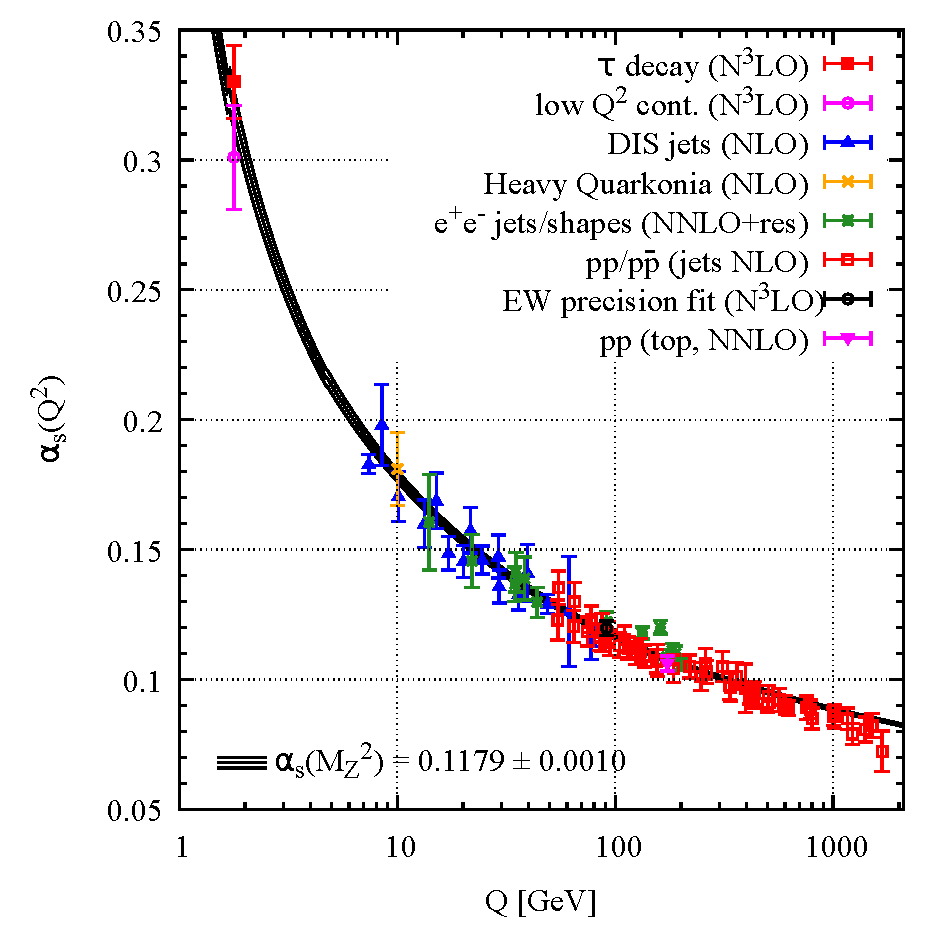
\includegraphics[width=0.7\textwidth]{Figures/Theory/SM/alphas_running.pdf}
  \caption[Measurements of $\alpha_s$ as a Function of Energy Scale]{Summary of measurements of $\alpha_s$ ($\alpha_s = g_s^2 / 4\pi$) as a function of the energy scale, $Q$, taken from Ref.~\cite{ParticleDataGroup:2020ssz}. Each set of coloured points corresponds to a different set of measurements and the degree of QCD perturbation theory used to extract $\alpha_s$ is indicated by the brackets in the legend. Further details about the measurements and $\alpha_s$ calculations can be found in Ref.~\cite{ParticleDataGroup:2020ssz}.}\label{fig:alphas_running}
\end{figure}

\subsubsection{Electroweak Gauge Theory}
In the SM, the electroweak bosons arise from an $\SU{2} \times \U{1}$ gauge symmetry of \LSM. The representation of some field, $\chi$, under \SU{2} is given by generators $\{T^a\}$, $a \in \{1,2,3\}$, and the generator of \U{1} can be any real number, $Y$, such that a gauge transformation is given by:
\begin{equation}
  \chi \to e^{i\theta^a T^a + i\eta Y} \chi
\end{equation}
where $\theta^a$ and $\eta$ are real numbers. The generators $T^a$ and $Y$ are called \textit{weak isospin} and \textit{weak hypercharge} respectively. The covariant derivative is given by:
\begin{equation}
  D_\mu = \partial_\mu + i g_2 A^a_\mu T^a + i g_1 Y B_\mu
  \label{eq:electroweak_covariant}
\end{equation}
where $A^a_\mu$ and $B_\mu$ are the \SU{2} and \U{1} gauge fields respectively. 

Experiments have measured the mass of the \PW and \PZ bosons to be non-zero~\cite{ParticleDataGroup:2020ssz} and in the SM, these masses are introduced via the Higgs mechanism. This necessitates electroweak theory to include a complex scalar field, $\phi$, which is the \textit{Higgs field}, and is in the fundamental representation of \SU{2} and $Y = 1/2$. By defining a fourth generator:
\begin{equation}
  t^4 = \frac{g_1}{2g_2} \iden,
\end{equation}
and $A_\mu^4 = B_\mu$, the gauge fields can be represented by a single vector field in the covariant derivative of the Higgs field:
\begin{equation}
  D_\mu \phi = \partial_\mu \phi + i g_2 A_\mu^{a'} t^{a'} \phi,
\end{equation}
which is useful for applying the ideas of the symmetry breaking matrix introduced in \cref{eq:symmetry_breaking_matrix}. The Lagrangian of the theory is:
\begin{equation}
  \mathcal{L} = -\frac{1}{2} \Tr W_\mn W^\mn - \frac{1}{4} F_\mn F^\mn + (D_\mu \phi)^\dag D^\mu \phi + \mu^2 \phi^\dag \phi - \lambda (\phi^\dag \phi)^2 
  \label{eq:electroweak_gauge_terms}
\end{equation}
where $W_\mn$ and $F_\mn$ are the field strength tensors of the \SU{2} and \U{1} gauge fields respectively. After electroweak symmetry breaking, the residual symmetry group is \U{1} and in terms of the original gauge fields, the physical gauge boson spectrum is:
\begin{align}
  \mathcal{A}_\mu &= \cos{\theta_W} B_\mu + \sin{\theta_W} A^3_\mu, &&\text{ with mass } m_\gamma = 0 \\
  W_\mu^\pm &= \frac{1}{\sqrt{2}} (A^1_\mu \mp i A^2_\mu), &&\text{ with mass } m_\PW = \frac{g_2 v}{2} \\
  Z_\mu &= \cos{\theta_W} A^3_\mu - \sin{\theta_W} B_\mu, &&\text{ with mass } m_\PZ = \frac{v}{2} \sqrt{g_1^2 + g_2^2 } 
\end{align}
which are the photon, \PWpm bosons, and \PZ boson respectively where $\theta_W$ is the Weinberg angle, and is related to $g_1$ and $g_2$ by:
\begin{equation}
  \sin{\theta_W} = \frac{g_1}{\sqrt{g_1^2 + g_2^2 }}\quad \text{and} \quad \cos{\theta_W} = \frac{g_2}{\sqrt{g_1^2 + g_2^2}} .
\end{equation}
In addition, the Higgs field gives rise to a physical scalar boson, the Higgs boson, with mass ${m_H = \sqrt{2} \mu}$. 

In the physical mass basis, the covariant derivative is written as:
\begin{equation}
  D_\mu = \partial_\mu + i \frac{g_1 g_2}{\sqrt{g_1^2 + g_2^2}}(T^3 + Y)\mathcal{A}_\mu + i \frac{g_2^2 T^3 - g_1^2 Y}{\sqrt{g_1^2 + g_2^2}} \PZ_\mu + \frac{ig_2}{\sqrt{2}} (\PW_\mu^+ T^+ + W_\mu^- T^-)
\end{equation}
where $T^\pm = T^1 \pm iT^2$. From the second term, we see that the electric charge, $e$, which characterizes the strength of interactions with photons, is given by:
\begin{equation}
  e = \frac{g_1 g_2}{\sqrt{g_1^2 + g_2^2}} = g_2 \sin{\theta_W} .
\end{equation}
The Weinberg angle can be determined by the ratio of the \PW and \PZ masses:
\begin{equation}
  \cos{\theta_W} = \frac{m_\PW}{m_\PZ} \approx \frac{80.377\GeV}{91.188\GeV} = 0.88145 \pm 0.00013 .
\end{equation}
The parameter, $e$, can be determined from the fine structure constant, $\alpha$:
\begin{equation}
  e = \sqrt{4\pi \alpha} \approx \sqrt{\frac{4\pi}{137}} \approx 0.30
\end{equation}
and the \SU{2} and \U{1} gauge couplings are:
\begin{equation}
  g_2 = \frac{e}{\sin{\theta_W}} \approx 0.64,\quad g_1 = \frac{e}{\cos{\theta_W}} \approx 0.34
\end{equation}
The Higgs vev, $v$, can be determined by the \PW boson mass:
\begin{equation}
  v = \frac{2m_\PW}{g_2} \approx 246\GeV
\end{equation}
and given a measurement of the Higgs boson mass, ${m_\PH = 125.38 \pm 0.14}$~\cite{CMS:2020xrn}, the Higgs self-coupling is determined:
\begin{equation}
  \lambda = \frac{m_H^2}{2v^2} \approx 0.13 .
  \label{eq:higgs_self_coupling}
\end{equation}

\subsubsection{Electroweak Interactions with Fermions}
The interactions of the fermions with the electroweak force are determined by the representation that the fermions take under the \SU{2} and \U{1} gauge transformations. Initially, we will consider only the first generation of fermions: the electron ($e$) and electron neutrino ($\nu$), and the up ($u$) and down ($d$) quarks. Since the weak interaction can change leptons into neutrinos and up into down quarks, left-handed fermions are written in doublets which are in the fundamental representation of \SU{2}:
\begin{equation}
  l_L = \begin{pmatrix}
    \nu_L \\ e_L 
  \end{pmatrix},\quad
  q_L = \begin{pmatrix}
    u_L \\ d_L
  \end{pmatrix}.
\end{equation}
The generators of \U{1}, $Y$, take the value of $-1/2$ and $1/6$ for the left-handed leptons and quarks respectively, where these values are determined by requiring that the fermions have the correct electric charges. Given that the right-handed fermions do not interact with the weak force, they are said be neutral under \SU{2} meaning they do not transform under \SU{2} and the corresponding generator is zero. Additionally, the right-handed neutrino is neutral under \U{1} since it has no electric charge. Therefore, it does not interact with any SM forces, and consequently, it is left out of the theory. The rest of the right-handed fermions are written as singlets, denoted by $e_R$, $u_R$ and $d_R$ and have $Y = -1, 2/3, \text{ and } -1/3$ respectively.

Terms involving fermions and the covariant derivative, referred to as kinetic terms, encode electroweak interactions in the Lagrangian and are:
\begin{equation}
  \LEW = \bar{l}_L i \slashed{D} l_L + \bar{e}_R i \slashed{D} e_R + \bar{q}_L i \slashed{D} q_L + \bar{u}_R i \slashed{D} u_R + \bar{d}_R i \slashed{D} d_R + \cdots
\end{equation}
where $D$ is the covariant derivative defined in \cref{eq:electroweak_covariant}. We must also add terms that encode the mass of the fermions. Since the left-handed and right-handed fermions transform differently under \SU{2} and \U{1}, mass terms like:
\begin{equation}
  -m(\bar{e}_L e_R + \bar{e}_R e_L)
\end{equation} 
are not gauge invariant and cannot be included in \LSM. Instead, the fermion masses are introduced via the Higgs field and spontaneous symmetry breaking similarly to how the gauge bosons acquired their masses. This is achieved with \textit{Yukawa} terms:
\begin{equation}
  \LEW = - y_e (\bar{l}_l \phi l_R + \bar{l}_R \phi^\dag l_L) -  y_u (\bar{q}_L \tilde{\phi} u_R + \bar{u}_R \tilde{\phi}^\dag q_L) - y_d (\bar{q}_l \phi d_R + \bar{q}_R \phi^\dag d_L) + \cdots
\end{equation}
where $y$ are real constants called \textit{Yukawa} couplings and $\tilde{\phi} \equiv i \sigma_2 \phi^*$. After spontaneous symmetry breaking, these terms become:
\begin{equation}
  \LEW = -\frac{y_e v}{\sqrt{2}}  (\bar{e}_L e_R + \bar{e}_R e_L) -\frac{y_u v}{\sqrt{2}}  (\bar{u}_L u_R + \bar{u}_R u_L) -\frac{y_d v}{\sqrt{2}}  (\bar{d}_L d_R + \bar{d}_R d_L) + \cdots
\end{equation}
which corresponds to masses of $y_e v / \sqrt{2}$, $y_u v / \sqrt{2}$ and $y_d v / \sqrt{2}$ for the electron and up and down quarks respectively. No mass term is given to the neutrino and it is therefore massless in the SM. Given the observation of neutrino oscillations~\cite{Super-Kamiokande:1998kpq}, we know that neutrinos are, in fact, not massless in nature, however, for the results discussed in the rest of this thesis, the neutrino masses are small enough that $m_\nu = 0$ is a safe assumption. Therefore, neutrino masses will not be discussed further.

Generalizing to three generations, we define three-component column vectors:
\begin{equation}
  L_L = \begin{pmatrix}
    l_L^1 \\
    l_L^2 \\
    l_L^3 
  \end{pmatrix}, \quad
  L_R = \begin{pmatrix}
    l_R^1 \\
    l_R^2 \\
    l_R^3 
  \end{pmatrix}, \quad
  Q_L = \begin{pmatrix}
    q_L^1 \\
    q_L^2 \\
    q_L^3
  \end{pmatrix}, \quad
  D_R = \begin{pmatrix}
    d_R^1 \\
    d_R^2 \\
    d_R^3 \\
  \end{pmatrix}, \quad
  U_R = \begin{pmatrix}
    u_R^1 \\
    u_R^2 \\
    u_R^3
  \end{pmatrix}
\end{equation}
and then write the kinetic and Yukawa terms as:
\begin{equation}
  \begin{gathered}
    \LEW = \bar{L}_L i \slashed{D} L_L + \bar{L}_R i \slashed{D} L_R + \bar{Q}_L i \slashed{D} Q_L + \bar{D}_R i \slashed{D} D_R + \bar{U}_R i \slashed{D} U_R \\
  - (\bar{L}_L Y_l \phi L_R + \bar{Q}_L Y_d \phi D_R + \bar{Q}_L Y_u \tilde{\phi} U_R + \text{h.c.}) + \cdots
  \end{gathered}
  \label{eq:electoweak_fermion_terms}
\end{equation}
where $Y_{l,d,e}$ are complex $3 \times 3$ Yukawa matrices and $\text{h.c.}$ corresponds to the Hermitian conjugate. By redefining the fermion fields such that the Yukawa matrices are diagonal, we can find the physical mass basis for the fermions. The fields would be redefined according to:
\begin{equation}
  \begin{gathered}
    L_L \to V_{lL} L_L, \quad L_R \to V_{lR} L_R, \quad U_R \to V_{uR}  U_R, \quad  D_R \to V_{dR} D_R, \\
  Q_L = \begin{pmatrix}
    U_L \\
    D_L   
  \end{pmatrix} \to 
  \begin{pmatrix}
    V_{uL} U_L \\
    V_{dL} D_L
  \end{pmatrix}
  \end{gathered}
  \label{eq:fermion_redefinitions}
\end{equation}
where the $V$ matrices are determined by singular value decomposition of the Yukawa matrices. For the leptons, this leaves the kinetic terms:
\begin{equation}
  \LEW =  \sum_f \bar{l}_L^f i \slashed{D} l_L + \bar{l}_R^f i \slashed{D} l_R^f + \cdots
\end{equation}
where $f \in \{e, \mu, \tau\}$, unchanged. Since the terms are the same across flavour, the leptons interact identically in the SM, and this is known as \textit{lepton universality}. Furthermore, the terms are invariant under transformations of the type:
\begin{equation}
  l_L^f \to e^{i\theta^f} l_L^f, \quad l_R^f \to e^{i\theta^f} l_R^f, \quad \theta^f \in \mathbb{R}
\end{equation}
meaning that there is a global $\U{1}_e \times \U{1}_\mu \times \U{1}_\tau$ symmetry. This symmetry corresponds to a conserved lepton number for each generation.

After the field redefinitions of \cref{eq:fermion_redefinitions}, the kinetic terms for the right-handed quarks remain the same in an analogous way to the leptons. However, the kinetic terms for the left-handed quarks do not if $V_{uL} \neq V_{dL}$. When writing the covariant derivative in the physical mass basis, we find that the photon and \PZ boson terms are the same as before. Therefore, interactions with photons and \PZ bosons are identical across quark generation. On the other hand, the \PW boson terms are changed. In terms of the redefined quark fields, the kinetic \PW boson term is:
\begin{equation}
  \LEW = - \frac{g_2}{\sqrt{2}} ( V^{fg}_{\text{CKM}} \bar{u}_L^f \gamma^\mu W_\mu^+ d_L^g + \text{h.c.} ) + \cdots
\end{equation}
where $V_{\text{CKM}} \equiv V_{uL}^\dag V_{dL}$ is the Cabibbo-Kobayashi-Maskawa (CKM) matrix. If $V_{\text{CKM}}$ is not diagonal, it allows the interaction between left-handed quarks and the \PW boson to change quark flavour. There are four free parameters of the CKM matrix which are three mixing angles: $\theta_{12}$, $\theta_{13}$, $\theta_{23}$, and a complex phase: $\delta$. These parameters have been measured and the corresponding CKM matrix is given by:
\begin{equation}
  V_{\text{CKM}} \approx
  \begin{pmatrix}
    0.974 & 0.227 & 0.004 \\
    0.226 & 0.973 & 0.041 \\
    0.009 & 0.040 & 0.999
  \end{pmatrix}
\end{equation}
where the magnitudes of each element, $|V_{\text{CKM}}^{fg}|$, are shown. This indicates that there are small levels of mixing between neighbouring generations, and even smaller mixing between the first and third generations.

The full electroweak Lagrangian is given by the combination of the gauge terms in \cref{eq:electroweak_gauge_terms} with the fermion terms in \cref{eq:electoweak_fermion_terms}:
\begin{align}
  \begin{split}
   \LEW = &-\frac{1}{2} \Tr W_\mn W^\mn - \frac{1}{4} F_\mn F^\mn \\ 
    &+ (D_\mu \phi)^\dag D^\mu \phi + \mu^2 \phi^\dag \phi - \lambda (\phi^\dag \phi)^2 \\
    &+ \bar{L}_L i \slashed{D} L_L + \bar{L}_R i \slashed{D} L_R + \bar{Q}_L i \slashed{D} Q_L + \bar{D}_R i \slashed{D} D_R + \bar{U}_R i \slashed{D} U_R \\
    &- (\bar{L}_L Y_l \phi L_R + \bar{Q}_L Y_d \phi D_R + \bar{Q}_L Y_u \tilde{\phi} U_R + \text{h.c.}) .
  \end{split}
  \label{eq:ew_lagrangian}
\end{align}

\subsubsection{The Standard Model Lagrangian}
To write the full SM Lagrangian, we combine \LEW with \LQCD to get:
\begin{align}
  \begin{split}
    \LSM = &- \frac{1}{4} G^{c\mn} G^c_\mn -\frac{1}{2} \Tr W_\mn W^\mn - \frac{1}{4} F_\mn F^\mn \\ 
    &+ (D_\mu \phi)^\dag D^\mu \phi + \mu^2 \phi^\dag \phi - \lambda (\phi^\dag \phi)^2 \\
    &+ \bar{L}_L i \slashed{D} L_L + \bar{L}_R i \slashed{D} L_R + \bar{Q}_L i \slashed{D} Q_L + \bar{D}_R i \slashed{D} D_R + \bar{U}_R i \slashed{D} U_R \\
    &- (\bar{L}_L Y_l \phi L_R + \bar{Q}_L Y_d \phi D_R + \bar{Q}_L Y_u \tilde{\phi} U_R + \text{h.c.})
  \end{split}
\end{align}
where the covariant derivative is:
\begin{equation}
  D_\mu = \partial_\mu + ig_s G^c_\mu \frac{\lambda^c}{2} + ig_2 A^a_\mu T^a + ig_1 Y B_\mu,
\end{equation}
and where the quark mass terms in \LQCD have been dropped since they are now accounted for with the Yukawa terms. In addition to the 18 free parameters mentioned already, there is also the strong CP phase, $\theta^{\text{CP}}$, that can lead to CP violation in the strong interaction. Experimentally, $\theta^{\text{CP}}$, is known to be very small, $\theta^{\text{CP}} \simeq 0$. More information about this parameter can be found in Ref.~\cite{Wu:1991rw}. All 19 free parameters of the SM are listed in \cref{tab:SM_free_parameters}.

\begin{table}
  \centering
  \begin{tabular}{r|l}
    \toprule
    Fermion masses & $m_u, m_c, m_t, m_d, m_s, m_b, m_e, m_\mu, m_\tau$ \\
    Gauge couplings & $g_s, g_1, g_2$ \\
    Higgs & $\lambda, \mu^2$ \\
    CKM & $\theta_{12}, \theta_{13}, \theta_{23}, \delta$ \\
    Strong CP phase & $\theta^{\text{CP}} (\approx 0)$ \\
    \bottomrule
  \end{tabular}
  \caption[Free Parameters in the SM]{The 19 free parameters of the SM.}\label{tab:SM_free_parameters}
\end{table}